\documentclass[12pt]{article}
\usepackage[utf8]{inputenc}
\usepackage[T1]{fontenc}
\usepackage{graphicx}
\usepackage{xcolor}
\usepackage{hyperref}

%%novalidate

\usepackage{tikz}
\usepackage{calc}
\usepackage{booktabs}
%\usepackage{hyperref}

% colors
\definecolor{color1}{HTML}{000060} % 19% Dark Blue
% \definecolor{color1}{HTML}{8C260F} % Dark red
\definecolor{color2}{HTML}{333333} % 20% gray
% \definecolor{color2}{HTML}{000060} % 19% Dark Blue
\definecolor{colorcover}{HTML}{333333} % 20% gray

% fonts
\usepackage{fontspec}
\defaultfontfeatures{Mapping=tex-text}
\setmainfont
[BoldFont=Lato-Bold.ttf,
ItalicFont=Lato-Italic.ttf,
BoldItalicFont=Lato-BoldItalic.ttf]
{Lato-Regular.ttf}
\newfontfamily\headingfont[ItalicFont=Lato-BlackItalic.ttf]{Lato-Black.ttf}
%%%

\usepackage{geometry}
\geometry{a4paper,
hmargin=20mm,vmargin=20mm,
head=0ex,foot=3ex}

\linespread{1.3}

\usepackage[hang]{caption}
\DeclareCaptionFormat{upper}{#1#2\uppercase{#3}\par}
\captionsetup{labelfont={bf,color=color2},textfont={normalsize,color=color2},format = upper,figurename=FIGURE,tablename=TABLE}

%%% fancy sections
\usepackage{titlesec}
%\titleformat{\chapter}{\headingfont\LARGE\bfseries\scshape\color{color1}}{\thechapter}{1em}{}[\titlerule]
\titleformat{\section}{\color{color1}\headingfont\Large\bfseries\uppercase}{\thesection}{1em}{}[\titlerule]
\titleformat{\subsection}{\color{color1}\headingfont\large\bfseries\uppercase}{\thesubsection}{1em}{}
\titleformat{\subsubsection}{\color{color1}\headingfont\bfseries\uppercase}{\thesubsubsection}{1em}{}
%%%

% head and foot
\usepackage{fancyhdr}
\pagestyle{fancy}
\lhead{}
\chead{}
\makeatletter
\rhead{\color{color2}\@date}
\makeatother
\newlength{\myheight}
\lfoot{
\settoheight{\myheight}{\thepage}
\raisebox{-2ex-0.5\myheight}{
\includegraphics[height=4ex]{logo}}
}
\cfoot{\color{color2} Free \LaTeX\ template for LGU reports}
\rfoot{\color{color2}\thepage}
\renewcommand\headrulewidth{0pt}
\renewcommand\footrulewidth{0pt}

%%% picture on cover page
\usepackage{eso-pic}
\newcommand\BackgroundPic{%
\put(0,0){%
\parbox[b][\paperheight]{\paperwidth}{%
\vfill
\centering

\includegraphics[width=\paperwidth,height=\paperheight,%
keepaspectratio]{cover}%
\vfill
}}
\put(0,0){%
\parbox[b][\paperheight]{\paperwidth}{%
\vfill
\centering

\includegraphics[width=0.5\paperwidth]{logo.png}%
\vfill
}}}
%%%
% custom titlepage
\makeatletter
\renewcommand{\maketitle}{
\thispagestyle{empty}
\AddToShipoutPicture*{\BackgroundPic}
\ClearShipoutPicture
%
\phantom{a}
\vfill
\phantom{a}\hfill
\begin{tabular}[c]{@{}p{0.7\textwidth}@{}}
      \color{colorcover}\headingfont\LARGE\@title\\[1em]
      \color{colorcover}\headingfont\Large\@author\\[2em]
\end{tabular}
%
\clearpage
}
\makeatother
%%%


%%% fancy boxes
\usepackage{tcolorbox}
\usepackage{wrapfig}
\def\fullboxbegin{
\bigskip
\begin{tcolorbox}[colback=color1,colframe=color1,coltext=white,arc=0mm,boxrule=0pt]
}
\def\fullboxend{\end{tcolorbox}\medskip}
%
\def\leftboxbegin{
\begin{wrapfigure}{l}{0.5\textwidth}
\begin{tcolorbox}[colback=color1,colframe=color1,coltext=white,arc=0mm,boxrule=0pt]
}
\def\leftboxend{
\end{tcolorbox}
\end{wrapfigure}
}
%
\def\rightboxbegin{
\begin{wrapfigure}{r}{0.5\textwidth}
\begin{tcolorbox}[colback=color1,colframe=color1,coltext=white,arc=0mm,boxrule=0pt]
}
\def\rightboxend{
\end{tcolorbox}
\end{wrapfigure}
}
%
\newcounter{frames}
\def\frameboxbegin#1{
\bigskip
\refstepcounter{frames}
\begin{tcolorbox}[colback=white,colframe=color1,arc=0mm,title={\MakeUppercase{\textbf{Frame \arabic{frames}}: #1}}]
}
\def\frameboxend{
\end{tcolorbox}
}
%%%

\usepackage{lipsum}

%%%%%%%%%%%%%%%
% Title Page
\title{Free \LaTeX\ template for LGU Reports}
\author{GX \newline 120000000 \newline gx@apartsa.com}
\date{\today}
%%%%%%%%%%%%%%%

\begin{document}
\maketitle

\tableofcontents
\clearpage

\section{Introduction}

\textbf{WARNING:} This template is for LGU reports. Please use the logo and icon \textbf{properly}. It is your responsibility to use them \textbf{legally}. If you are using this template outside LGU, please contact the university for its permission or remove them.

The main purpose of this template is a free template to get start your academic reports with one click. Anyone can reproduce this template and create their own styles based on this one, as long as referencing this template. This template is based on \href{https://www.overleaf.com/latex/templates/another-template-for-business-reports/jjqkjjmcptkg}{\textit{Another template for business reports}}.

To contact me, send to my email on the cover page. Welcome any suggestions and requirements! Join our tutorials by emailing me!

\section{Get Started}

\subsection{Sections}

You can insert a new section, subsection, or subsubsection using the commands:

\begin{verbatim}
    \section{Section Name}
    \subsection{Subsection Name}
    \subsubsection{Subsubsection Name}
\end{verbatim}

Note: the table of content will update simultaneously.

\subsection{New Page}
If you want to insert a new page, use the command \begin{verbatim}
    \newpage
\end{verbatim}

\subsection{Text formatting}

Two useful text formatting commands are \textbf{BOLD} and \textit{Italics}. \textbf{PS: you can also use CTRL (Command) + B and CTRL (Command) + I in Overleaf.} 

\begin{verbatim}
    \textbf{BOLD}
    \textit{Italics}.
\end{verbatim}

\subsection{Inserting Images}

Examples of inserting a single image or two images in a row:
\begin{figure}[!h]
    \centering
    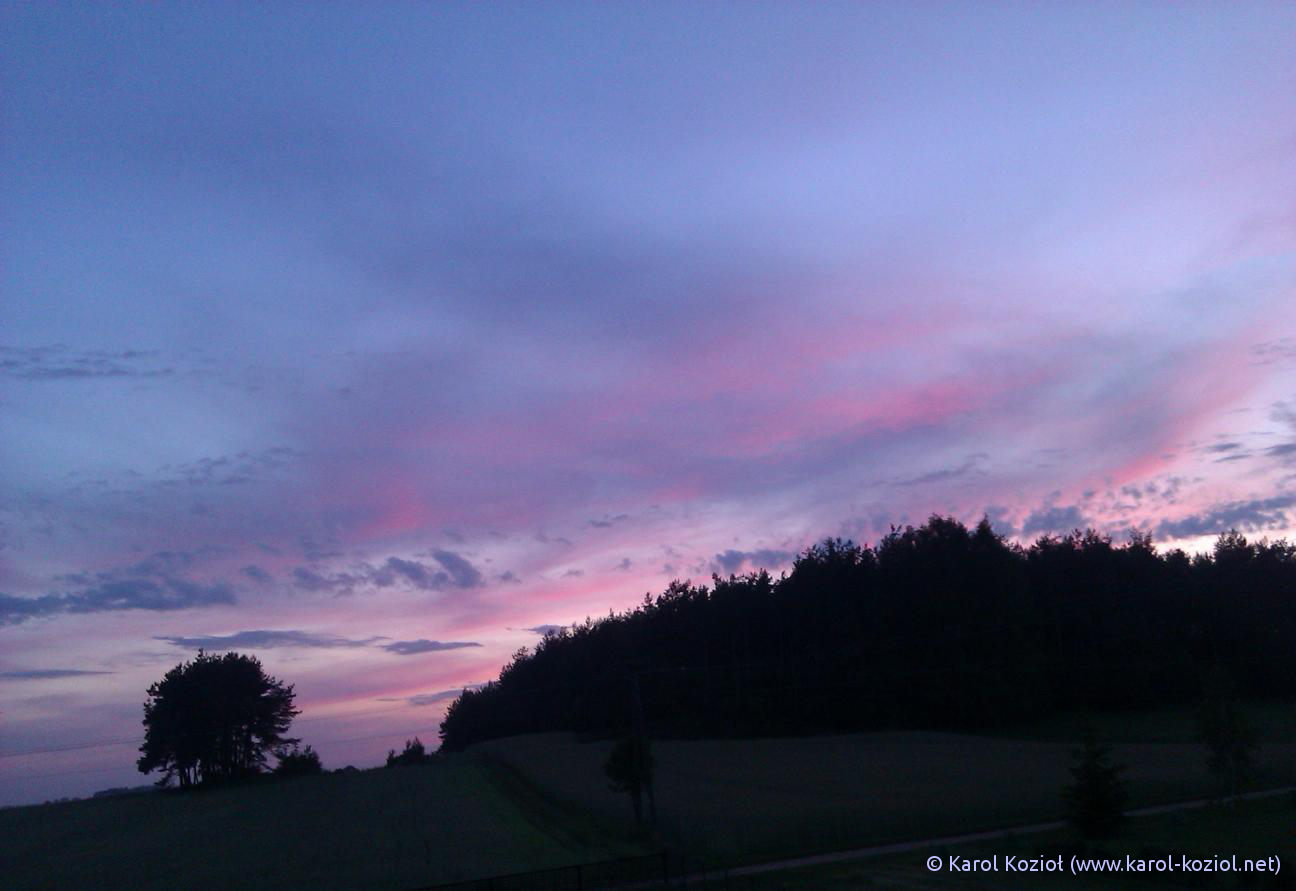
\includegraphics[width=0.5\textwidth]{sky.jpg}
    \caption{The sky is the limit.}
\end{figure}

\begin{figure}[!h]
\centering
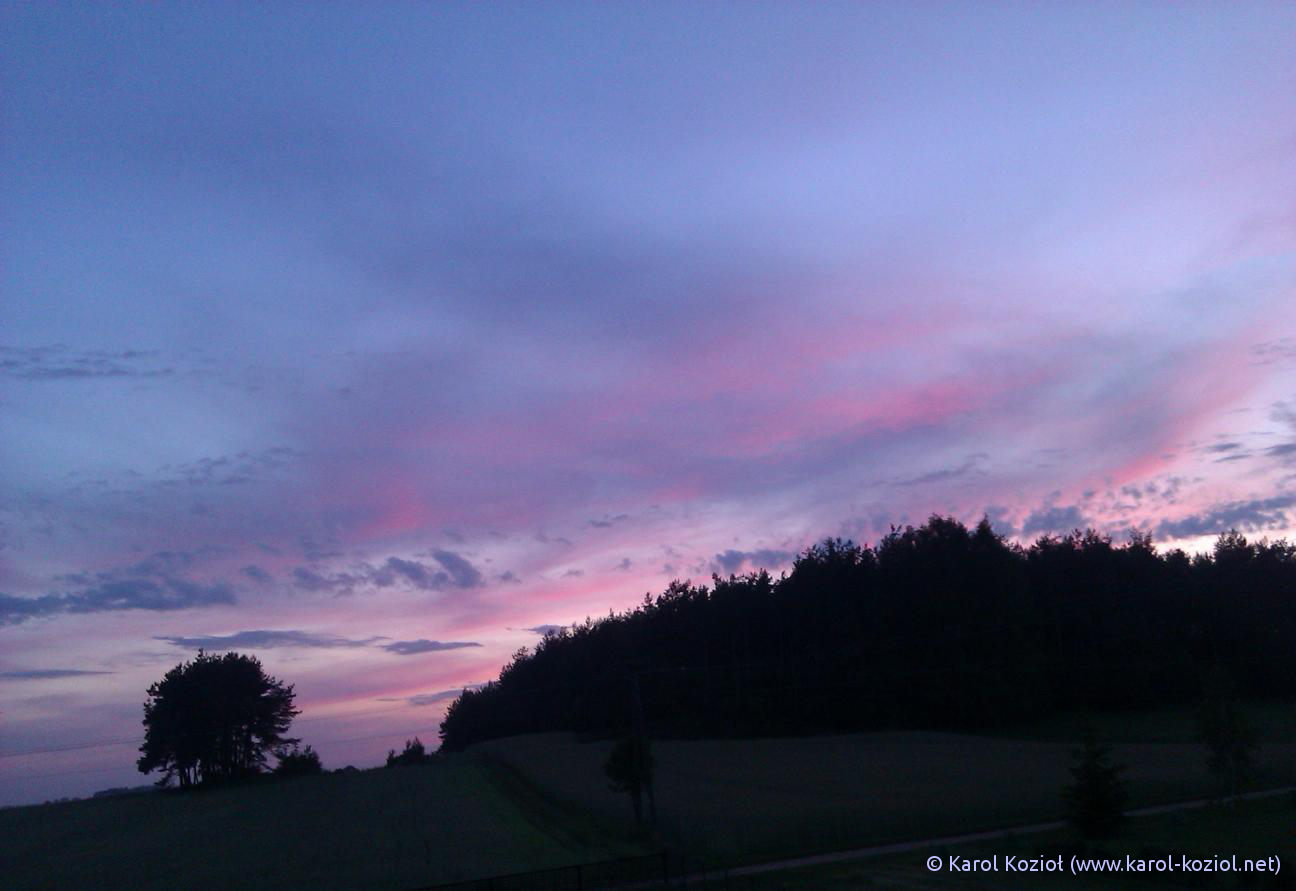
\includegraphics[width=0.5\textwidth]{sky.jpg}
\caption*{The sky is the limit. (No prefix)}
\end{figure}

\begin{figure}[htbp]
    \centering
    \begin{minipage}[t]{0.48\textwidth}
        \centering
        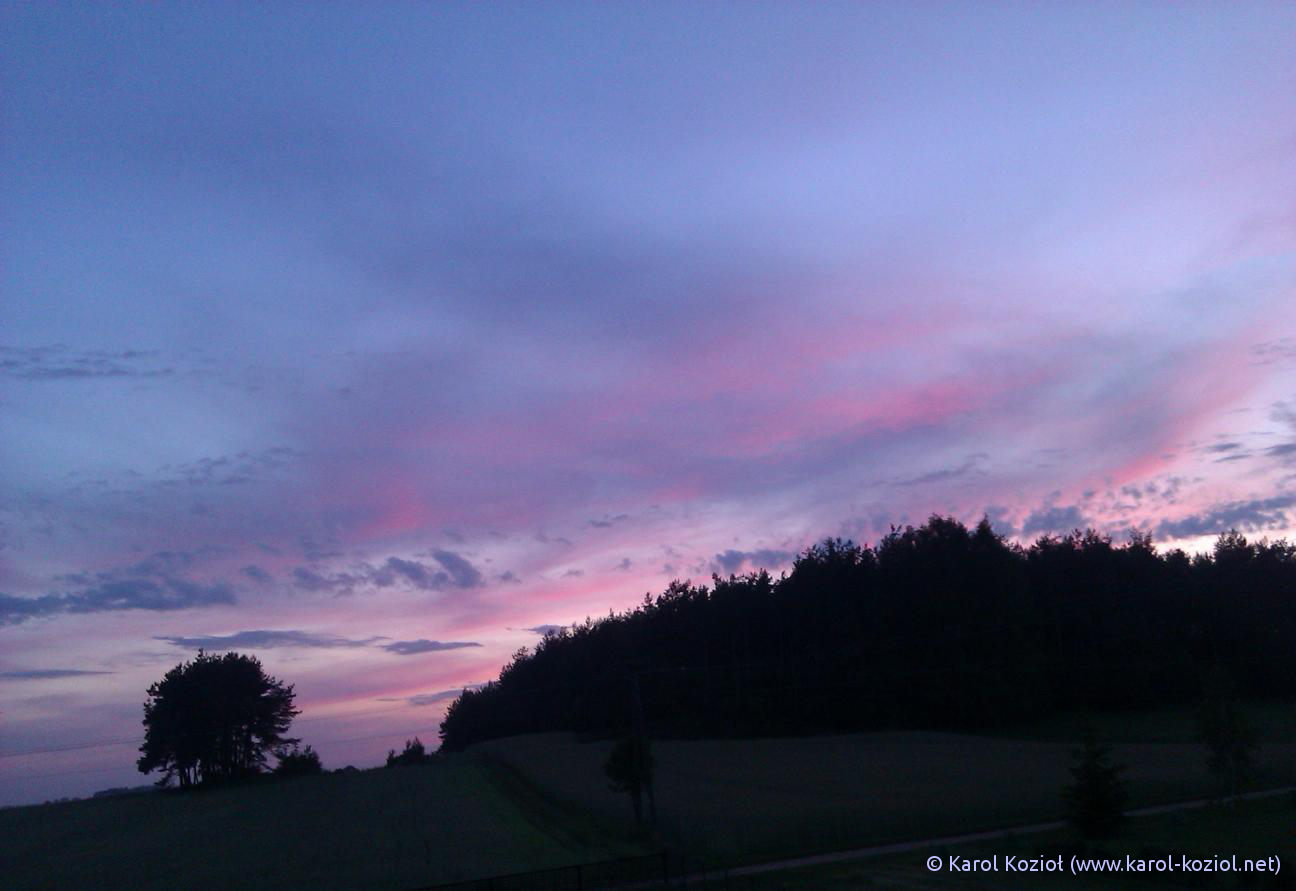
\includegraphics[width=\textwidth]{sky.jpg}
        \caption{LEFT}
    \end{minipage}
    \begin{minipage}[t]{0.48\textwidth}
        \centering
        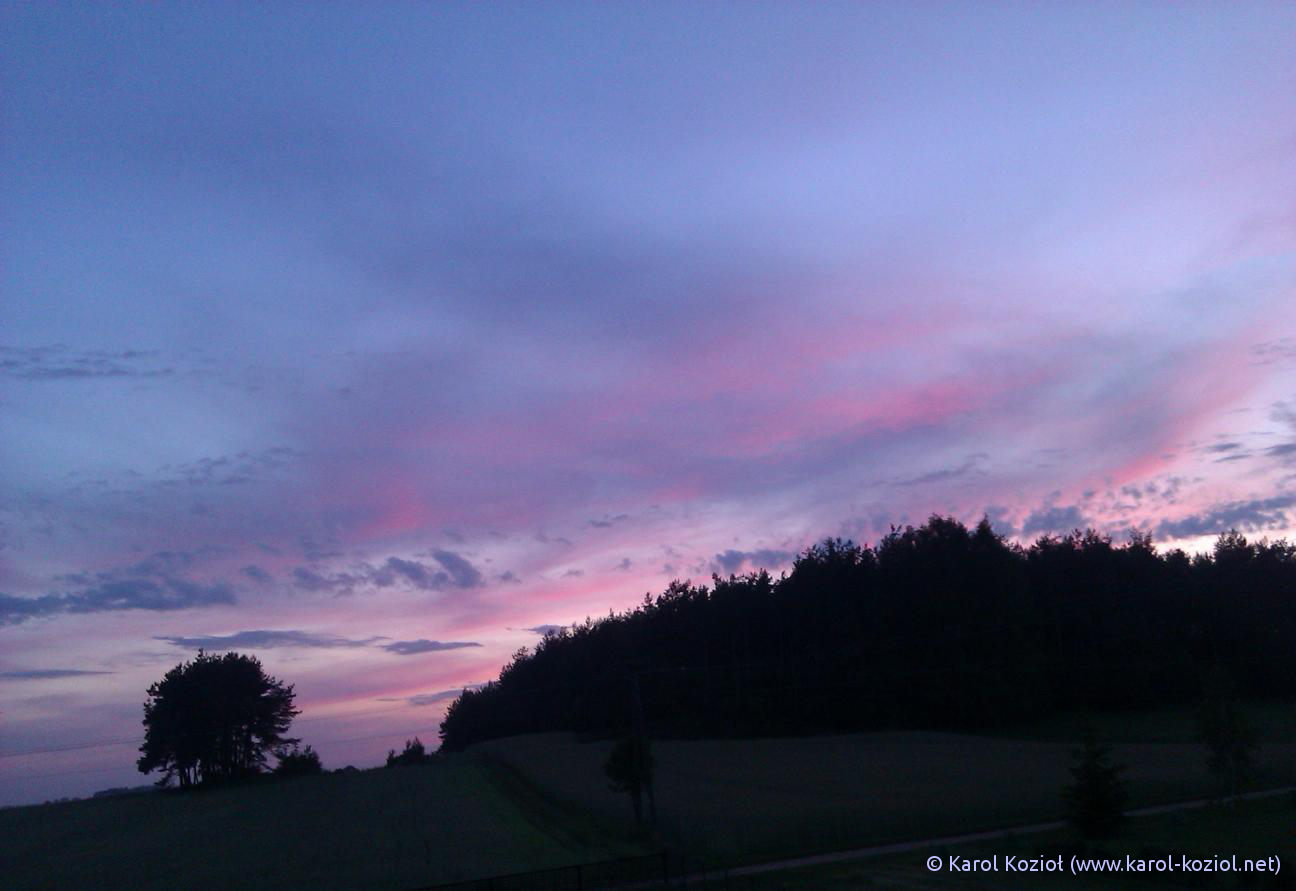
\includegraphics[width=\textwidth]{sky.jpg}
        \caption{RIGHT}
    \end{minipage}
\end{figure}

\begin{verbatim}
    \begin{figure}[!h]
        \centering
        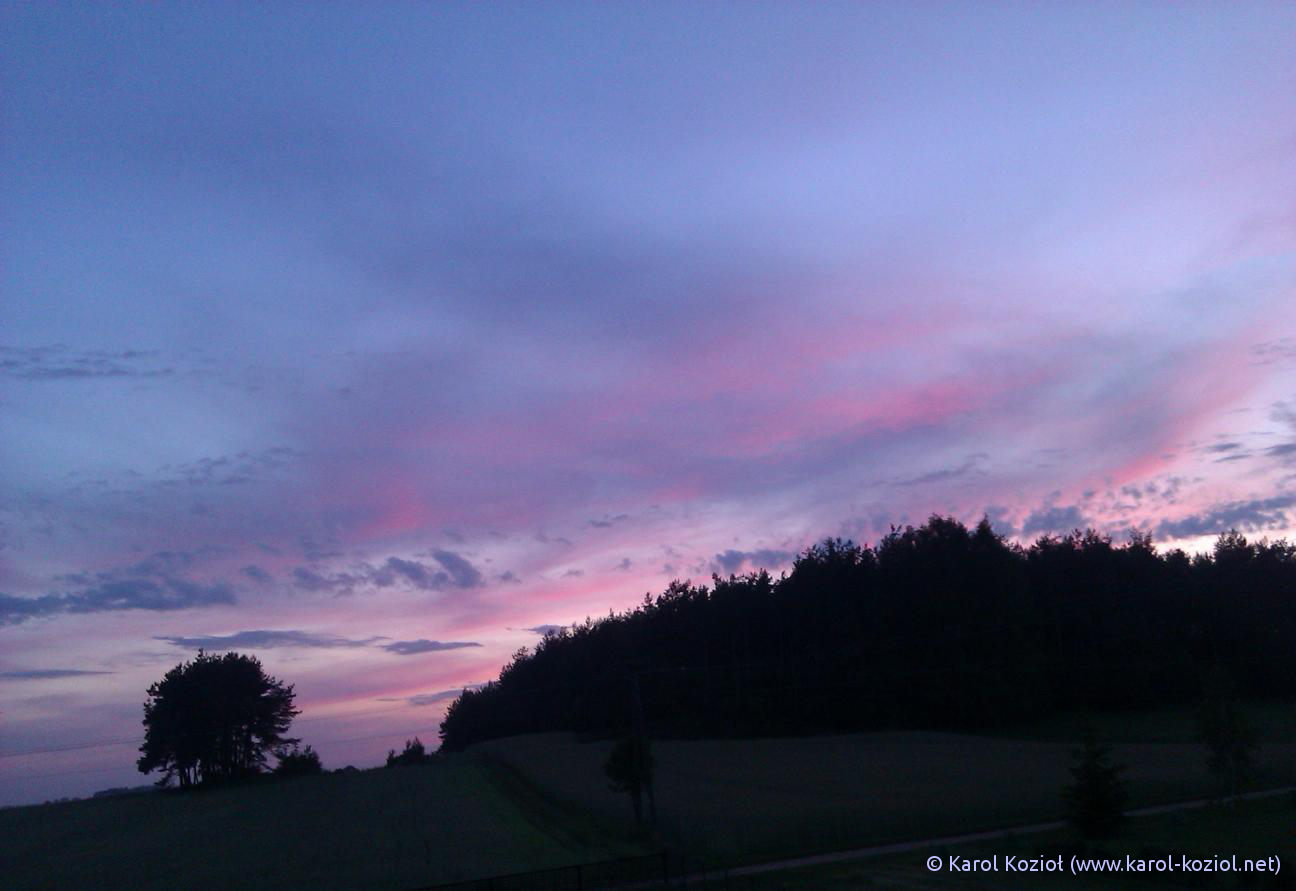
\includegraphics[width=0.5\textwidth]{sky.jpg}
        \caption{The sky is the limit.}
    \end{figure}
    
    \begin{figure}[!h]
        \centering
        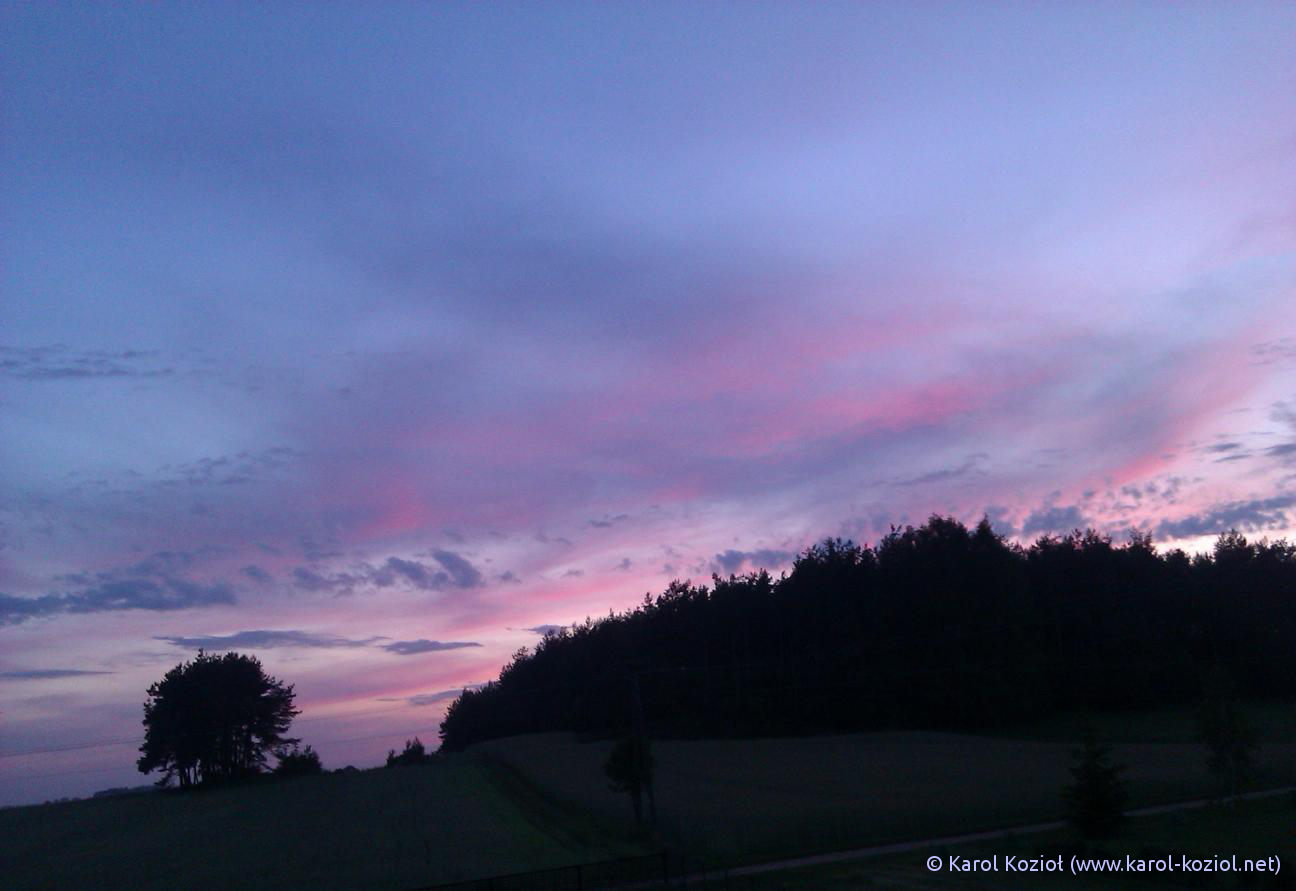
\includegraphics[width=0.5\textwidth]{sky.jpg}
        \caption*{The sky is the limit. (No prefix)}
    \end{figure}
    
    \begin{figure}[htbp]
        \centering
        \begin{minipage}[t]{0.48\textwidth}
            \centering
            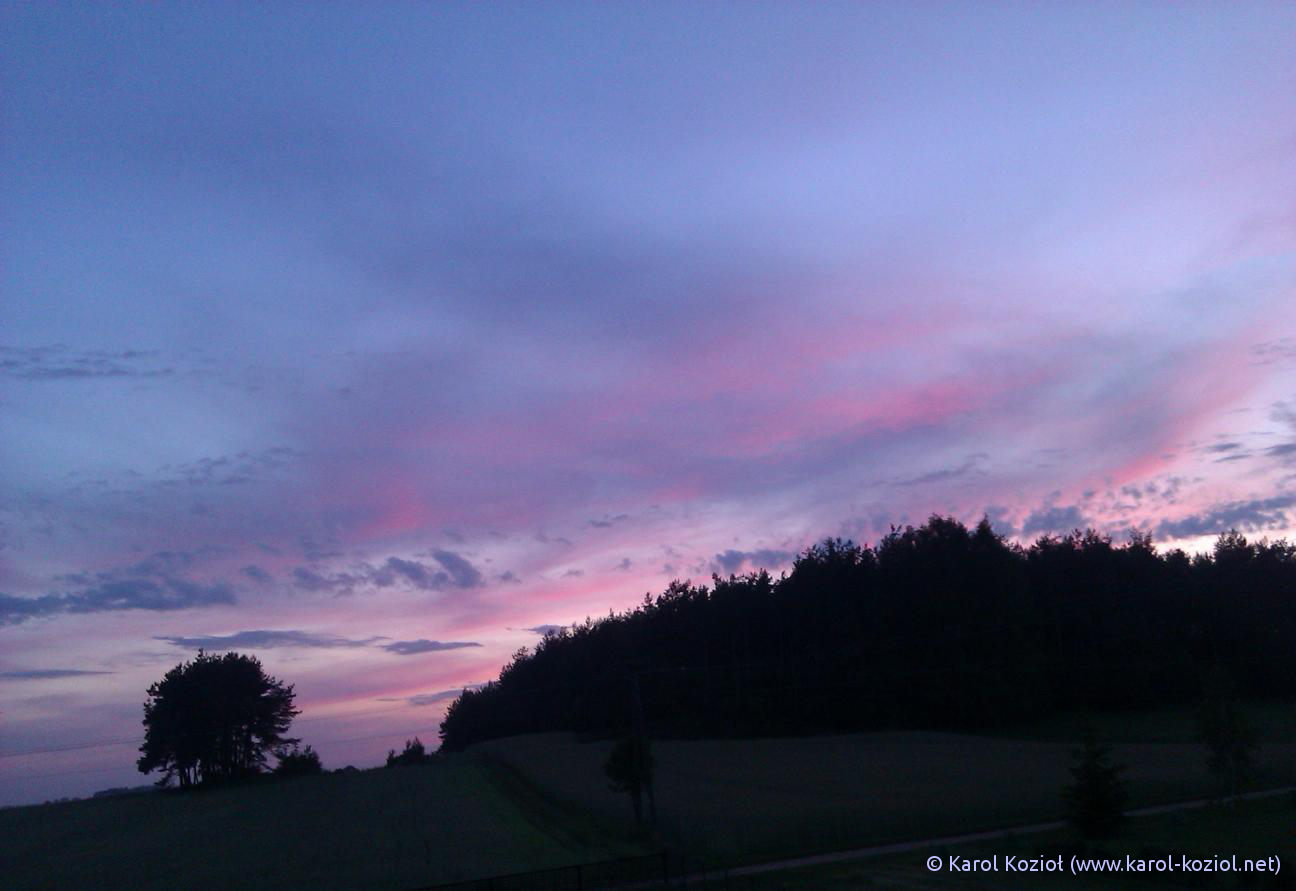
\includegraphics[width=\textwidth]{sky.jpg}
            \caption{LEFT}
        \end{minipage}
        \begin{minipage}[t]{0.48\textwidth}
            \centering
            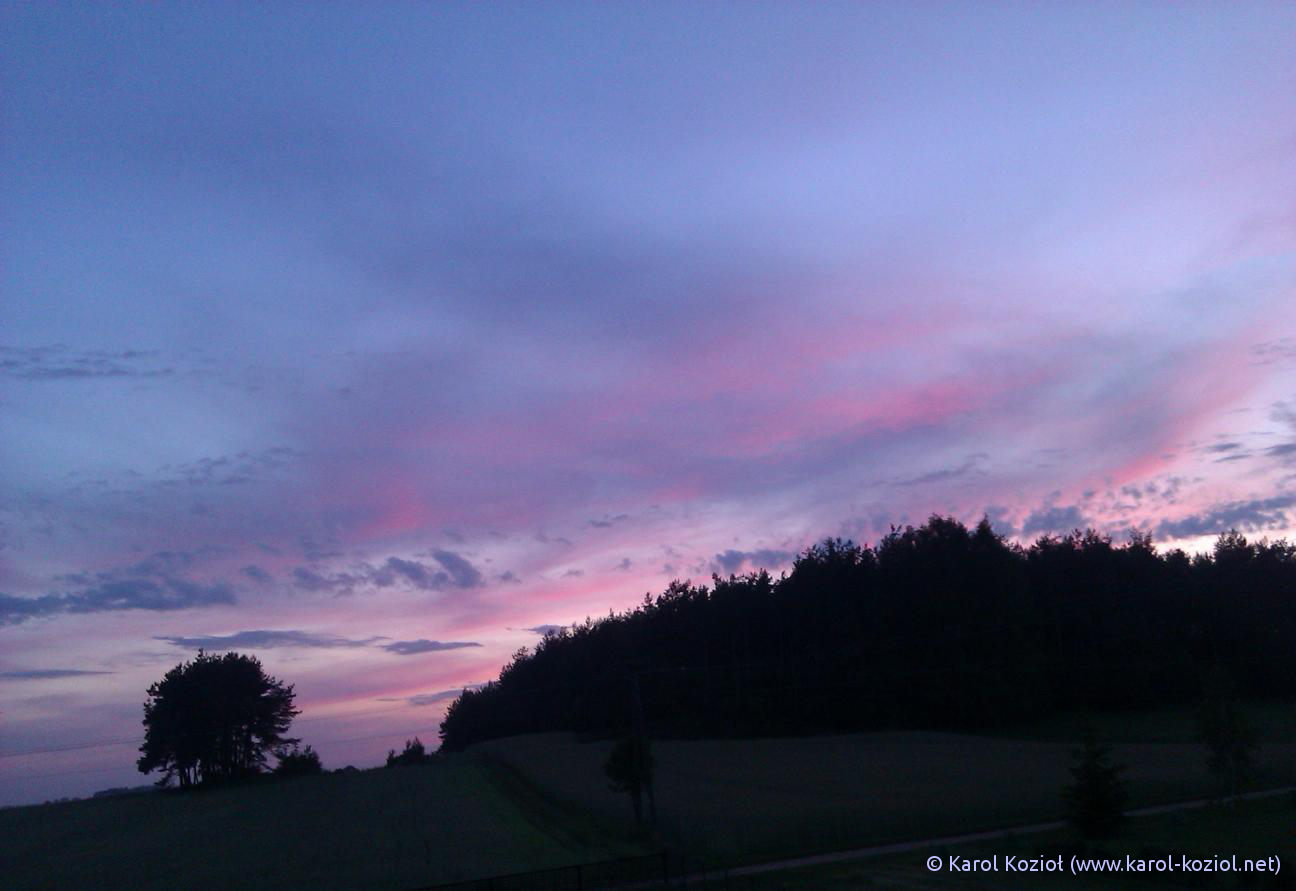
\includegraphics[width=\textwidth]{sky.jpg}
            \caption{RIGHT}
        \end{minipage}
    \end{figure}
\end{verbatim}

\subsection{Tables}

\begin{table}[!h]
\centering
\caption{Sample table.}
\begin{tabular}{cccc}
\toprule
Value 1 & Value 2 & Value 3 & Value 4\\
\midrule
 odd     & odd   & odd & 1.00 \\
 even    & even  & even& 1.00 \\
 odd     & odd   & odd & 1.00 \\
 even    & even  & even& 1.00 \\
\bottomrule
\end{tabular}
\end{table}

\begin{verbatim}
    \begin{table}[!h]
        \centering
        \caption{Sample table.}
        \begin{tabular}{cccc}
        \toprule
        Value 1 & Value 2 & Value 3 & Value 4\\
        \midrule
         odd     & odd   & odd & 1.00 \\
         even    & even  & even& 1.00 \\
         odd     & odd   & odd & 1.00 \\
         even    & even  & even& 1.00 \\
        \bottomrule
        \end{tabular}
    \end{table}
\end{verbatim}

\section{Features commands}

\subsection{Pictures used}

\noindent
Cover picture filename (in titlepage): \texttt{cover}\\
Cover logo filename (in titlepage): \texttt{lgu-logo}\\
Logo filename (in foot): \texttt{logo}

\subsection{Boxes}

\begin{verbatim}
\fullboxbegin
Content
\fullboxend
\end{verbatim}

\begin{verbatim}
\leftboxbegin
Content
\leftboxend
\end{verbatim}

\begin{verbatim}
\rightboxbegin
Content
\rightboxend
\end{verbatim}

\begin{verbatim}
\frameboxbegin{Frame Title}
Content
\frameboxend
\end{verbatim}

\subsection{Colors}
You can define \textbf{color1}, \textbf{color2}, and \textbf{colorcover} in \textit{defs.tex}. \textbf{color1} is used for \textbf{titles}, \textbf{color2} is used for headers and footers, and \textbf{colorcover} is used for the cover.

\newpage

\section{First section}
\lipsum[1]

\fullboxbegin
\lipsum[1]
\fullboxend

\lipsum[1]

\subsection{First subsection}
\lipsum[1]

\leftboxbegin
Lorem ipsum dolor sit amet, consectetuer adipiscing elit. Ut purus elit, vestibulum ut, placerat ac, adipiscing vitae, felis. Curabitur dictum gravida mauris. Nam arcu libero, nonummy eget, consectetuer id, vulputate a, magna. Donec vehicula augue eu neque. 
\leftboxend

\lipsum[1-2]

\rightboxbegin
\begin{itemize}
 \item Lorem ipsum
 \item Lorem ipsum
\end{itemize}
\rightboxend

\lipsum[1]

\subsubsection{First subsubsection}

\lipsum[1]

\section*{Unnumbered section}
\lipsum[1]



\frameboxbegin{Sample frame}
\lipsum[1]
\frameboxend

\newpage

\section{Architecture Design}
\lipsum[1]

\section{Experiment and Results}
\lipsum[1]

\section{Conclusion}
\lipsum[1]

\end{document}          
